\documentclass[10pt]{beamer}
\usetheme{PaloAlto}
\usecolortheme{seahorse}
\setbeamertemplate{navigation symbols}{}
\setbeamertemplate{caption}[numbered]
%general package
%\usepackage[utf8]{inputenc}
\usepackage[english]{babel}
\usepackage{geometry}
\usepackage{tcolorbox}
\usepackage[cmtip,all]{xy}
\newcommand{\longsquigarrow}{\xymatrix{{}\ar@{~>}[r]&{}}}
\usepackage[export]{adjustbox}
\usepackage{graphicx}
\graphicspath{{../img/}}
\usepackage{graphbox}
%math package
\usepackage{amsmath}
\usepackage{amsfonts}
%\usepackage{amssymb}
%\usepackage{amsthm}
%\usepackage{slashed}
%\usepackage{tikz-cd}
%\usepackage{extarrows}
%font package
\usepackage{mathrsfs}
%\usepackage{bm}
%\usepackage{thmtools}
%misc. package
\usepackage{enumitem}

\author[B.H.]{{\Large MATH211 Calculus III}\\\vspace{6pt}Instructor: Ben Huang}
\date{}
\title[Section 13.7]{Section 13.7 
Tangent Planes and Normal Lines}
\institute[MU]{
\includegraphics[width = 0.382\textwidth]{MCLogo-Bck.png}}
\logo{
\includegraphics[scale = 0.3]{MCLogo-Bck.png}}
%general package
\usepackage[utf8]{inputenc}
\usepackage[english]{babel}
\usepackage{geometry}
\usepackage{comment}

%math package
\usepackage{amsmath}
\usepackage{amsfonts}
\usepackage{amssymb}
\usepackage{amsthm}
\usepackage{slashed}
\usepackage{tikz-cd}
\usepackage{mathtools}

%font package
\usepackage{mathrsfs}
\usepackage{bm}

%misc. package
\usepackage{enumitem}
\usepackage{tcolorbox}
\usepackage{etoolbox}
\usepackage{hyperref}
\hypersetup{
  colorlinks=true, urlcolor=blue
}




%declared operators
\DeclareMathOperator{\id}{Id}%identity
\DeclareMathOperator{\ind}{Ind\!}%index
\DeclareMathOperator{\tr}{Tr}%trace
\DeclareMathOperator{\e}{e}%exponential
\DeclareMathOperator{\im}{Im\!}%image
\DeclareMathOperator{\vol}{vol}%volume
\DeclareMathOperator{\cll}{\C\ell}%complexified Clifford algebra
\DeclareMathOperator{\gd}{\slashed{\partial}}%geometric Dirac
\DeclareMathOperator{\D}{\mathcal{D}}%generalized Dirac
\DeclareMathOperator{\Div}{div}%divergence
\DeclareMathOperator{\ud}{\,\mathrm{d}\!}

\DeclareMathOperator{\Hom}{Hom}
\DeclareMathOperator{\xd}{\,d\!}
\DeclareMathOperator{\curl}{curl}
\DeclareMathOperator{\dive}{div}
\DeclareMathOperator{\proj}{proj}


\newcommand{\norm}[1]{\lVert#1\rVert}
\newcommand{\R}{\mathbb R}
\newcommand{\vF}{\mathbf F}
\newcommand{\vv}{\mathbf v}
\newcommand{\inpr}[1]{\left\langle#1\right\rangle}
\newcommand{\fix}{(a,b)}
\newcommand{\uv}{\mathbf u}
\newcommand{\abs}[1]{\lvert #1\rvert}
%texting in citation
\makeatletter
\let\cite\relax
\DeclareRobustCommand{\cite}{%
  \let\new@cite@pre\@gobble
  \@ifnextchar[\new@cite{\@citex[]}}
\def\new@cite[#1]{\@ifnextchar[{\new@citea{#1}}{\@citex[#1]}}
\def\new@citea#1{\def\new@cite@pre{#1}\@citex}
\def\@cite#1#2{[{\new@cite@pre\space#1\if\relax\detokenize{#2}\relax\else, #2\fi}]}
\makeatother

\begin{document}

\frame{\titlepage}
\begin{frame}
\frametitle{Tangent Plane}
\begin{tabular}{cc}
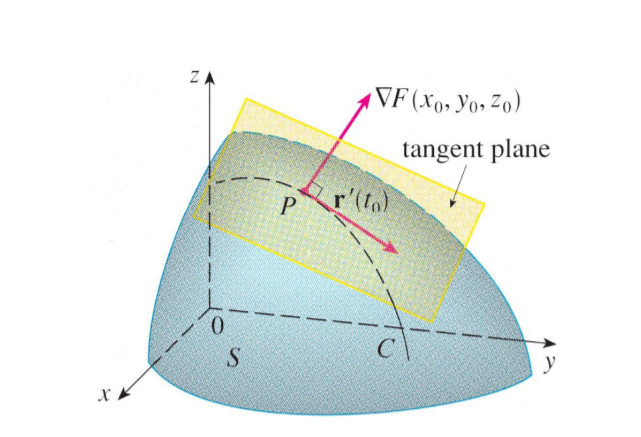
\includegraphics[width=.55\textwidth]{gradientAndCurve.png}&\pause
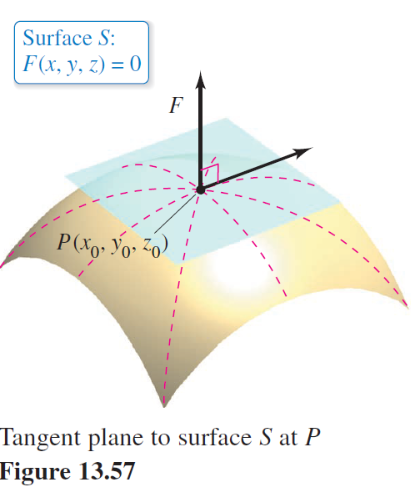
\includegraphics[width=.35\textwidth]{tanplane1.png}
\end{tabular}
\end{frame}
\begin{frame}
\frametitle{Why Tangent Plane?}
\pause
\begin{tabular}{cc}
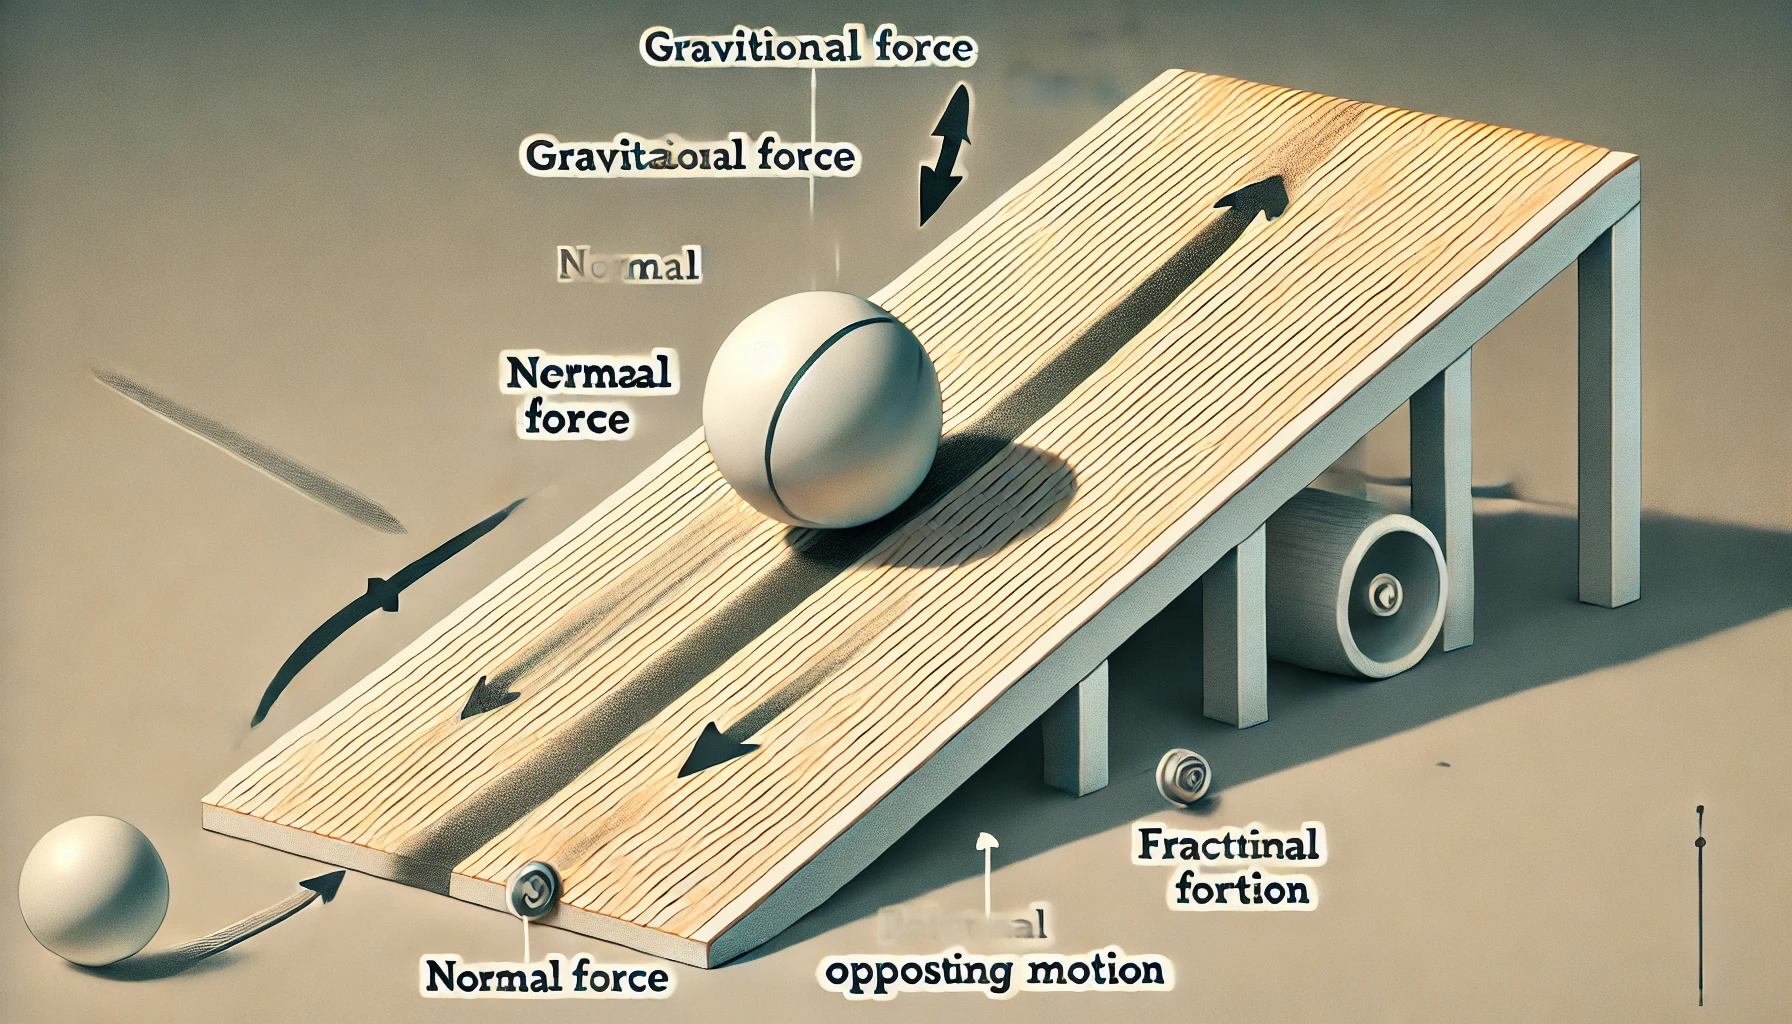
\includegraphics[width=.45\textwidth]{flatRamp.png}&\pause
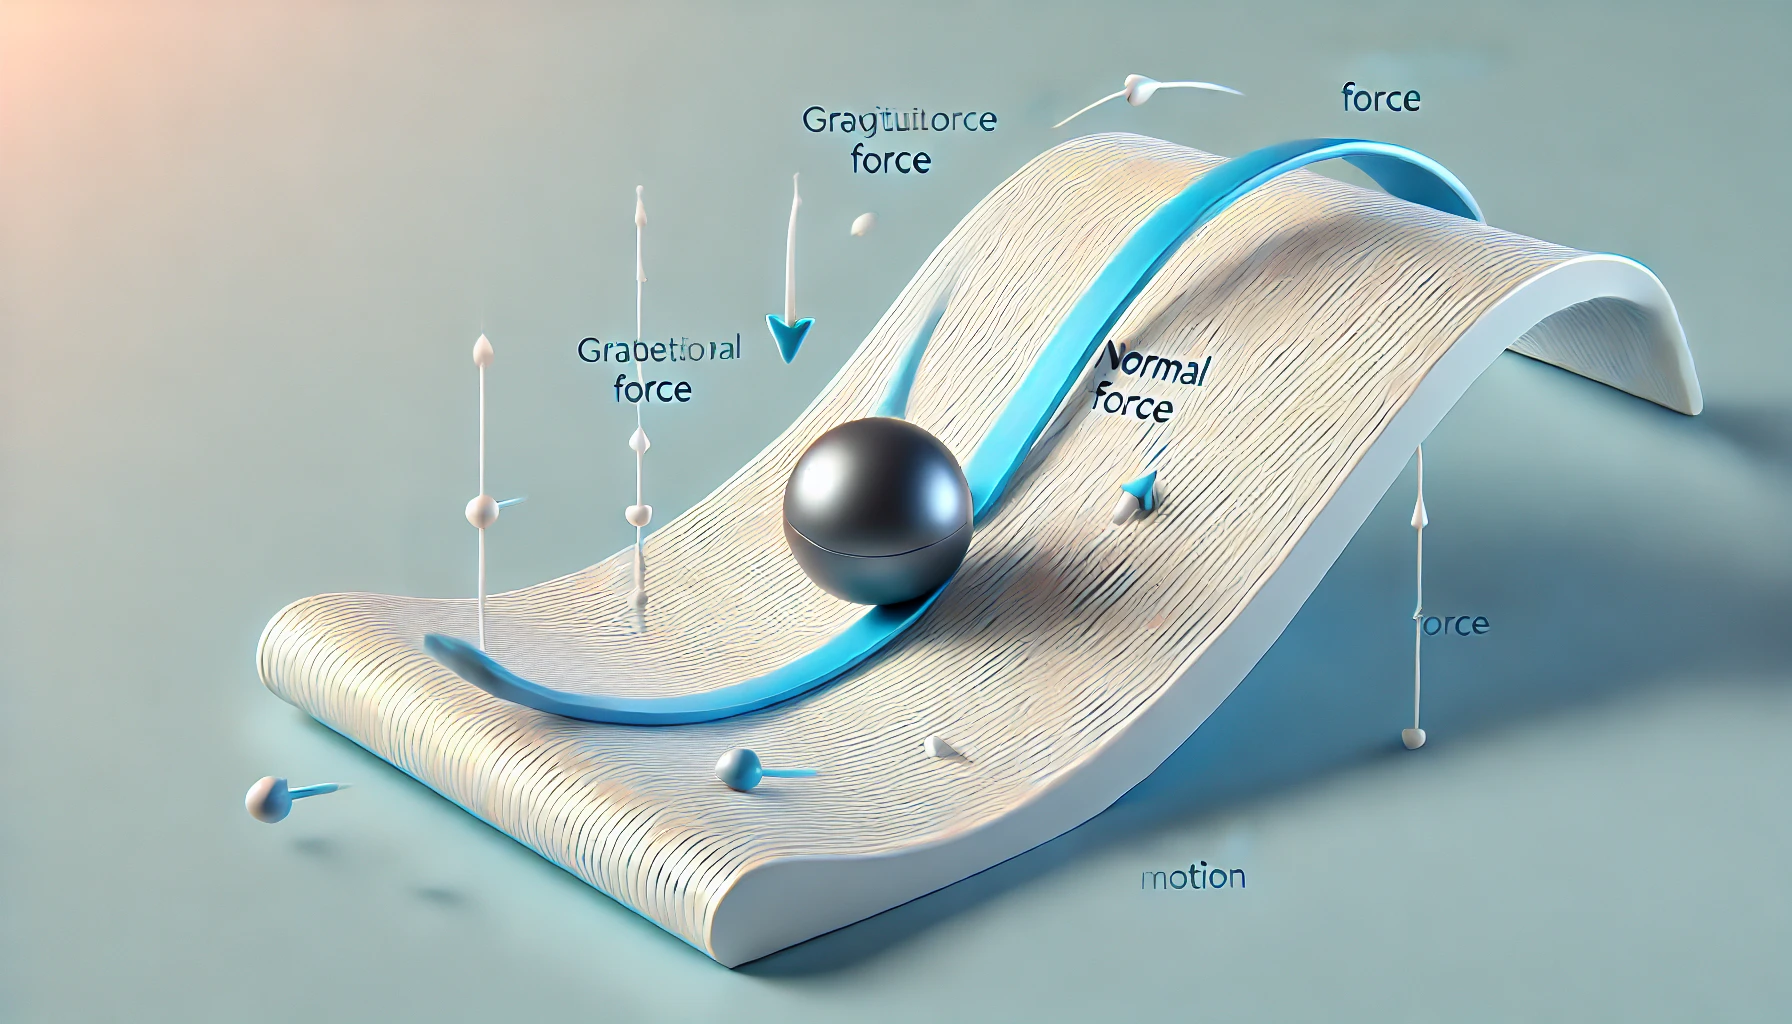
\includegraphics[width=.45\textwidth]{curvedRamp.png}
\end{tabular}
\end{frame}
\begin{frame}
\frametitle{Why Tangent Plane?}
\begin{tabular}{cc}
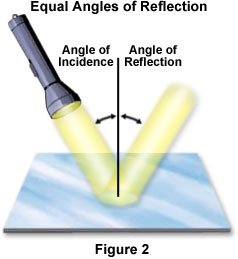
\includegraphics[width=.45\textwidth]{flatMirror.jpg}&\pause
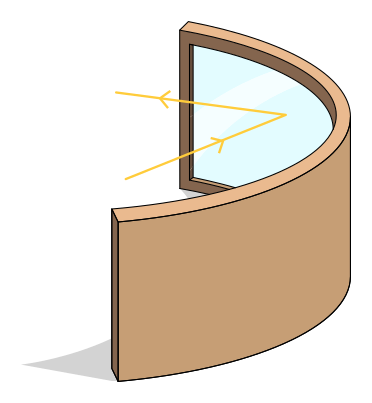
\includegraphics[width=.45\textwidth]{curvedMirror.png}
\end{tabular}
\end{frame}
\end{document}